\begin{frame}{Проблемное поле}
    \svg{sqeq}
\end{frame}

\begin{frame}{Целевая аудитория}
    \begin{itemize}
        \item<+-> Получающие знания:
            \begin{itemize}
                \item Школьники
                \item Студенты
            \end{itemize}
        \item<+-> Передающие знания:
            \begin{itemize}
                \item Преподаватели (учителя)
                \item Репетиторы
                \item Авторы учебников
                \item Составители учебных программ
            \end{itemize}
    \end{itemize}
\end{frame}

\begin{frame}{Способ решения}
    \svg{sqeq}
    % не запутаться по мере изучения. структурировать процесс изучения
\end{frame}

\begin{frame}{Некоторые термины}
    \begin{columns}[c]
        \begin{column}{.45\textwidth}
            \only<1>{
            \begin{tabular}{c}
                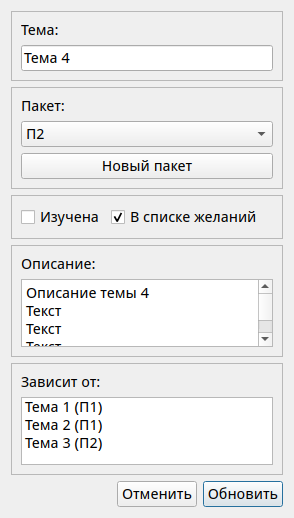
\includegraphics[height=0.70\textheight]{themeDialog}\\
                \includesvg[height=0.20\textheight]{edge}
            \end{tabular}
            }
            \only<2>{
                \svg{graph}
            }
            \only<3>{
                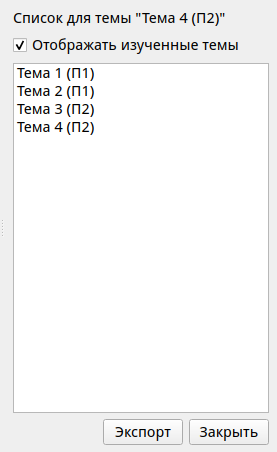
\includegraphics[height=0.7\textheight]{learningList}
            }
        \end{column}
        \begin{column}{.45\textwidth}
            \begin{itemize}
                \item<1-> Тема
                \item<1-> Пакет
                \item<1-> Ребро
                \item<2-> Граф
                \item<3-> Список изучения
            \end{itemize}
        \end{column}
    \end{columns}
\end{frame}

\begin{frame}{Образ продукта и окончательный продукт}
    \begin{itemize}
        \item<1-> Создать/ удалить/ изменить тему/ пакет/ граф
        \item<2-> Вывести отфильтрованый список тем/ пакетов/ графов % TODO: отфильтроваый
        \item<3-> Экспортировать темы/ список изучения/ пакеты/ граф
        \item<3-> Импортировать пакеты/ граф
        \item<4-> {\color{blue}Редактировать граф в визуальном режиме}
        \item<5-> Вывести список изучения для данной темы
        \item<6-> {\color{blue}Полу}автоматически сгенерировать пакет на основе сайта Wikipedia
        \item<7-> \textit{Функциональный интерфейс}
            % в интерфейсе программы присутствует много мелких функций, которые делают работу интуитивной и комфортной
        \item<8-> \textit{Синхронизация данных во всех рабочих областях программы}
            % изм-я происходящие с каким-то элементом происходят во всех частях программы и соотв. отобр
            % компонент
            % Синхронность работы частей программы
    \end{itemize}
\end{frame}

\begin{frame}{Аналогичные продукты}
    \begin{itemize}
        \item<1-> Учебники % нужно читать весь; нередактируется
        \item<2-> Статьи % предполагается знание других тем
        \item<3-> \url{graphonline.ru} % нет описания и генерации; другая задача
        \item<3-> \url{csacademy.com/app/graph\_editor} % нет описания и генерации; другая задача
        \item<3-> \url{webgraphviz.com} % написание кода и нет генерации, описания
    \end{itemize}
\end{frame}

\begin{frame}{Аппаратные требования и инструменты разработки}
    \begin{itemize}
        \item<+-> Операционная система: Linux
        \item<+-> Язык программирования: C++
        \item<+-> Графическая библиотека: Qt6
        \item<+-> База данных: SQLite3 \\
            Таблицы:
            \begin{itemize}
                \item packages
                \item themes
                \item themeEdges
                \item graphs
                \item graphNodes
                \item listThemes
            \end{itemize}
    \end{itemize}
\end{frame}

\begin{frame}{Демонстрация продукта}
    \img{demo}
\end{frame}

\begin{frame}{Возникшие проблемы и их решения}
    \begin{itemize}[<+->]
        \item Проблема --- нехватка времени
            \begin{itemize}
                \item Сложность совмещения с учебой
                \item Снижение мотивации
                \item Нехватка опыта на начальных этапах разработки
            \end{itemize}

        \item Решения:
            \begin{itemize}
                \item Перераспределение времени
                \item Техника Pomodoro
            \end{itemize}
    \end{itemize}
\end{frame}

\begin{frame}{Приобретенные навыки}
    \begin{itemize}[<+->]
        \item Навыки работы с:
        \begin{itemize}
            \item Библиотекой Qt 
            \item Базами данных (SQLite3)
        \end{itemize}
        \item Опыт создания большого программного продукта
    \end{itemize}
\end{frame}

\begin{frame}{Возможное развитие продукта}
    \begin{itemize}[<+->]
        \item Портирование на другие ОС
        \item Добавление других источников для генерации
        \item Улучшение дизайна приложения
    \end{itemize}
\end{frame}

\begin{frame}{Конец презентации}
    \img{demo}
\end{frame}
